\section{Diseño}

\begin{figure}
	\centering
	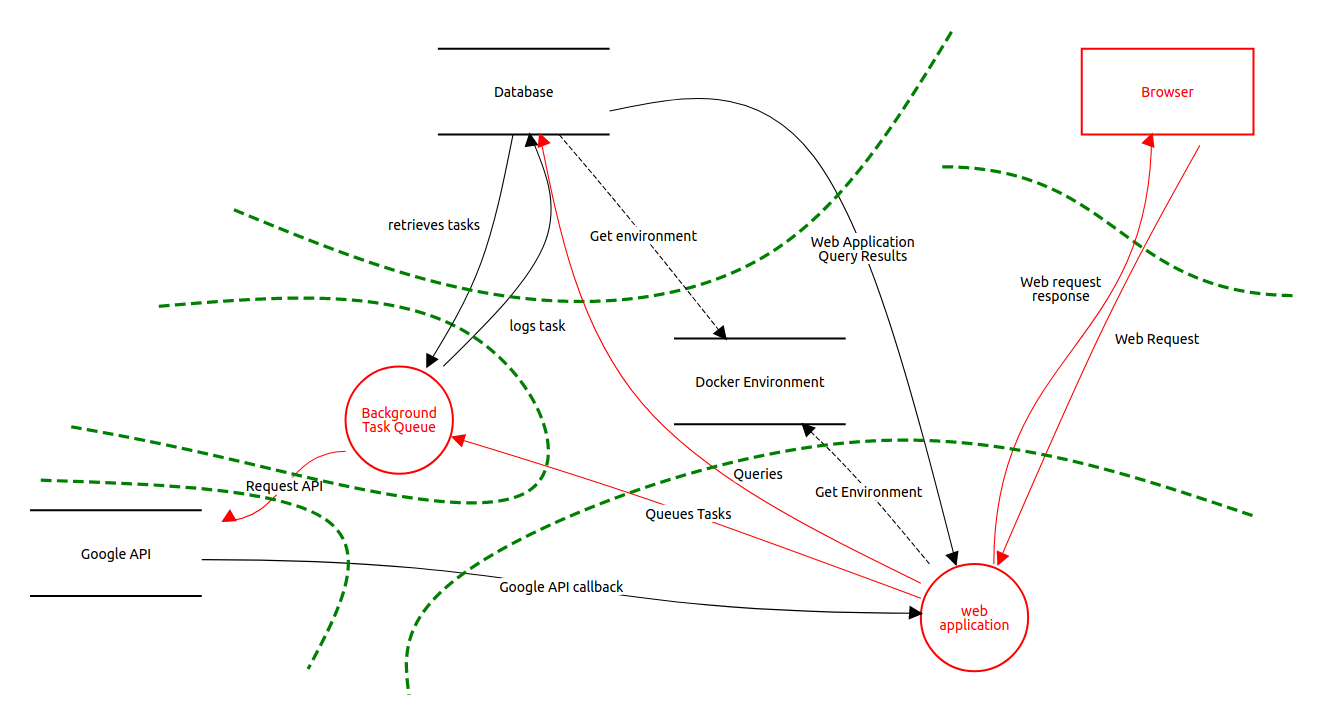
\includegraphics[width=.9\textwidth]{fragments/diagram.png}
	\caption{ Diagrama de modelo de riesgos generado por OWASP Dragon }
\end{figure}

Para el modelado de los riesgos utilizamos OPWASP Dragon debido a su facil integracion con las herramientas existentes y para poder dejar registro en el fork del repositorio original.

\subsection{Objetivos de seguridad}
Debido al contexto en el cual fue desarrollado este proyecto se asumieron los siguientes factores respecto del desarrollo:

\begin{itemize}
    \item El proyecto tendría continuidad por una tercera parte.
    \item Sus desarrolladores no tienen el nivel suficiente de madurez para desarrollar de manera segura.
\end{itemize}

Debido a esto, la mayor parte de los aspectos de seguridad son tratados durante la etapa de desarrollo por medio de prácticas estándarizadas de desarrollo, el uso correcto de herramientas y frameworks y un proceso auditable. 

En este marco de trabajo nuestro objetivo de seguridad se vuelve asegurar el acceso y disponibilidad del servicio y sus componentes a un mínimo aceptable para que una tercera parte pueda continuar el desarrollo sin mayores problemas.

\subsection{Activos y dependencias externas}

Los activos de información encontrados en esta aplicación si bien solo son de una única categoría pueden ser divididos de la siguiente forma:

\begin{itemize}
    \item{ Esquemas de almacenaje, que definen el como se estructura un elemento de evaluación. Estos pueden ser esquemas de:
        \begin{itemize}
            \item Preguntas de selección multiple
            \item Campos de Texto
            \item Resultados de encuestas
            \item Selectores
        \end{itemize}
    }
    \item{ Esquemas de presentación, que definen el como se estructura un elemento de presentación. Estos pueden ser esquemas de:
        \begin{itemize}
            \item Preguntas de selección multiple
            \item Campos de Texto
            \item Resultados de encuestas
            \item Selectores
            \item Metricas
            \item Indicadores
        \end{itemize}
    }
    \item{ Esquemas de cálculo, que definen el como se estructura el cálculo de un indicador o una métrica.}
    \item { Base de datos de usuarios }
\end{itemize}

Por otro lado, tenemos una dependencia externa implícita y otra explícita. De manera implícita, hay información que es depositada y consumida hacia bases de datos estructuradas como google docs, mientras que por otro lado tenemos una dependencia explícita de las estructuras entregadas a través de los documentos físicos a los desarrolladores para realizar el poblado inicial de la base de datos.

\subsection{Zonas de confianza}

Debido a las descisiones de implementación (que serán revisadas mas adelante) contamos con seis zonas de confianza bien definidas.

\begin{itemize}
    \item Base de datos
    \item Proceso para tareas de segundo plano
    \item Browser
    \item Aplicación web
    \item Api Google
    \item Red docker
\end{itemize}

De estas, la red de docker es quizás la única que no es obvia de observar en el diagrama. La razón es porque la infraestructura al ser montada sobre contenedores de docker tanto su aplicación principal, el servidor estático como la base de datos, permite establecer un control total de las comunicaciones ejecutadas como también de los permisos entregados a esta.

Adicionalmente por la naturaleza stateless de la aplicación, en si la red docker entrega una zona de confianza en un anillo mas bajo que el espacio de usuario, sin embargo, este espacio está reservado y sin acceso desde alguna parte de la aplicación. Debido a esto es que también el ambiente de docker se considera como un ambiente fuera del alcance.

Por otro lado, tenemos tareas de segundo plano que son ejecutadas dentro el mismo ambiente pero bajo una api diferente. Estas pertenecen a una API provista por un equipo externo al de desarrollo la cual fue impuesta como requisito para realizar labores de autenticación.

\subsection{Amenazas, vulnerabilidades y mitigaciones}

A continuación mencionaremos brevemente las amenazas, vulnerabilidades y mitigaciones que pueden ser identificadas al contrastar este modelo con el resto del desarrollo. Para esto, utilizamos el modelo STRIDE por la simpleza para este caso. Solo se considerarán riesgos que pueden ser de interés para este informe.

\subsubsection{Navegador - Actor Externo}
Intervención por 3ras personas
\begin{itemize}
    \item \textbf{Amenaza: } Tampering, revelación de información
    \item \textbf{Estado: } Abierto
    \item \textbf{Severidad: } Media
    \item \textbf{Descripción: } A nivel de navegador, este puede ser intervenido por medio de plugins de terceros para alterar el funcionamiento del frontend.
    \item \textbf{Mitigación: } Educar al usuario. No es mucho lo que se puede hacer desde el púnto de vista técnico para una aplicación que es ejecutada del lado del cliente.
\end{itemize}

\subsubsection{Aplicación Web - Proceso}
Auto-Tampering
\begin{itemize}
    \item \textbf{Amenaza: } Tampering
    \item \textbf{Estado: } Mitigado
    \item \textbf{Severidad: } Media
    \item \textbf{Descripción: } Malas prácticas de programación pueden alterar la integridad de los procesos o la información
    \item \textbf{Mitigación: } Verificación constante de prácticas de programación, implementación de code reviews constantes.
\end{itemize}

Repudio
\begin{itemize}
    \item \textbf{Amenaza: } Repudio
    \item \textbf{Estado: } Mitigado
    \item \textbf{Severidad: } Alta
    \item \textbf{Descripción: } Problemas genéricos de repudio de información
    \item \textbf{Mitigación: } Verificación de operaciones criticas como transacciones.
\end{itemize}


Elevación de privilegio
\begin{itemize}
    \item \textbf{Amenaza: } Elevación de privilegio
    \item \textbf{Estado: } Mitigado
    \item \textbf{Severidad: } Alta
    \item \textbf{Descripción: } Problemas genéricos de escalamiento de permisos
    \item \textbf{Mitigación: } Limitar permisos de ejecución y limpieza de entradas.
\end{itemize}


\subsubsection{Petición web - Flujo de datos}
Denegación de servicio
\begin{itemize}
    \item \textbf{Amenaza: } Denegación de servicio
    \item \textbf{Estado: } Mitigado
    \item \textbf{Severidad: } Media
    \item \textbf{Descripción: } Denegación de servicio generico por sobrecarga de requests
    \item \textbf{Mitigación: } Autoescalado
\end{itemize}

Ataque lateral
\begin{itemize}
    \item \textbf{Amenaza: } Tampering
    \item \textbf{Estado: } Abierto
    \item \textbf{Severidad: } Media
    \item \textbf{Descripción: } Zero-days
\end{itemize}


\subsubsection{Cola de tareas- Proceso}
Colisión de tareas
\begin{itemize}
    \item \textbf{Amenaza: } Tampering
    \item \textbf{Estado: } Abierto
    \item \textbf{Severidad: } Media
    \item \textbf{Descripción: } Tareas enconladas en estado huérfano
\end{itemize}

Errores no propagados
\begin{itemize}
    \item \textbf{Amenaza: } Repudio
    \item \textbf{Estado: } Abierto
    \item \textbf{Severidad: } Media
    \item \textbf{Descripción: } Al ocurrir un error en un proceso de segundo plano, este no es informado a la aplicación web
\end{itemize}

Denegación de servicio
\begin{itemize}
    \item \textbf{Amenaza: } Denegación de servicio
    \item \textbf{Estado: } Mitigado
    \item \textbf{Severidad: } Media
    \item \textbf{Descripción: } Denegación de servicio generico por sobrecarga de requests
    \item \textbf{Mitigación: } Limitación de recursos y tareas concurrentes
\end{itemize}

Elevación de privilegio
\begin{itemize}
    \item \textbf{Amenaza: } Elevación de privilegio
    \item \textbf{Estado: } Mitigado
    \item \textbf{Severidad: } Alta
    \item \textbf{Descripción: } Problemas genéricos de escalamiento de permisos
    \item \textbf{Mitigación: } Limitar permisos de ejecución y limpieza de entradas.
\end{itemize}


\subsubsection{API de request google- Flujo de datos}
Fuga de información
\begin{itemize}
    \item \textbf{Amenaza: } Fuga de datos
    \item \textbf{Estado: } Mitigado
    \item \textbf{Severidad: } Alta
    \item \textbf{Descripción: } Un ataque MitM puede ocasionar una fuga de información
    \item \textbf{Mitigación: } Trafico debe estar establecido por SSL sobre certificados verificados previamente intercambiados.
\end{itemize}

Denegación de servicio
\begin{itemize}
    \item \textbf{Amenaza: } Denegación de servicio
    \item \textbf{Estado: } Abierto
    \item \textbf{Severidad: } Medio
    \item \textbf{Descripción: } Denegación de servicio causada por un abuso del plan gratuito
\end{itemize}


\subsubsection{API callback google- Flujo de datos}
Fuga de información
\begin{itemize}
    \item \textbf{Amenaza: } Fuga de datos
    \item \textbf{Estado: } Mitigado
    \item \textbf{Severidad: } Alta
    \item \textbf{Descripción: } Protocolos inseguros de transporte
    \item \textbf{Mitigación: } Forzar utilización de HTTPS/2
\end{itemize}

\subsubsection{Respuesta servicio web - Flujo de datos}
Fuga de información
\begin{itemize}
    \item \textbf{Amenaza: } Fuga de datos
    \item \textbf{Estado: } Mitigado
    \item \textbf{Severidad: } Alta
    \item \textbf{Descripción: } Protocolos inseguros de transporte
    \item \textbf{Mitigación: } Forzar utilización de HTTPS/2
\end{itemize}


Explotación
\begin{itemize}
    \item \textbf{Amenaza: } Elevación de privilegio, Fuga de información, Tampering
    \item \textbf{Estado: } Mitigado
    \item \textbf{Severidad: } Alta
    \item \textbf{Descripción: } Explotación por medio de ZeroDay
\end{itemize}


\subsubsection{Queries - Flujo de datos}
Fuga de información
\begin{itemize}
    \item \textbf{Amenaza: } Fuga de datos
    \item \textbf{Estado: } Mitigado
    \item \textbf{Severidad: } Alta
    \item \textbf{Descripción: } Inyecciones SQL
    \item \textbf{Mitigación: } Limpieza forzada de consultas
\end{itemize}


\subsection{Vista general de la aplicación}